
% IKNP03 https://www.iacr.org/archive/crypto2003/27290145/27290145.pdf
% Nie07  "Extending Oblivious Transfers Efficiently How to get Robustness Almost for Free"
% KOS15  https://eprint.iacr.org/2015/546.pdf
% OOS16  https://eprint.iacr.org/2016/933.pdf

\newcommand{\rr}{\ensuremath{\boldsymbol{r}}}
\renewcommand{\tt}{\ensuremath{\boldsymbol{t}}}
\newcommand{\ww}{\ensuremath{\boldsymbol{w}}}
\newcommand{\cc}{\ensuremath{\boldsymbol{c}}}
\newcommand{\uu}{\ensuremath{\boldsymbol{u}}}
\newcommand{\qq}{\ensuremath{\boldsymbol{q}}}
\newcommand{\bb}{\ensuremath{\boldsymbol{b}}}
\newcommand{\vv}{\ensuremath{\boldsymbol{v}}}
\newcommand{\nc}{\ensuremath{{n_\mathcal{C}}}}
\newcommand{\kc}{\ensuremath{{k_\mathcal{C}}}}
\newcommand{\dc}{\ensuremath{{d_\mathcal{C}}}}

\section{OT Extension}


In this section we explore the rich implications endemic OT has on efficient 1-out-of-$N$ OT extension along with presenting two new attacks and fixes of existing uniform\footnote{\cite{KOS15, OOS16} refer to uniform OT as random OT $\mathcal{F}^{m,\kappa}_{\textsf{ROT}}$} OT extension protocols\cite{KOS15, OOS16}. These protocols are derived from the seminal black-box protocol of Ishia, Kilian, Nissim and Petrank\cite{IKNP03} and we note that in all cases the Sender Chosen Message variant of these protocols\cite{IKNP03, KOS15, OOS16} are secure. In particular, these Sender Chosen Message protocol perform the following transformations $\OOT^\send\overset{\pi_1}{\rightarrow} \OOT^\E \overset{\pi_2}{\rightarrow} \OOT^\send$. However, as we will explore next, \figureref{fig:OTExtrelations} suggestions a more efficient transformation exists where $\pi_1$ takes $\OOT^\E$ as input.

%Our new endemic OT protocol of \sectionref{sec:endemicOT} along with the variants satisfying different message security notions can be 

%used to \emph{securely} run the protocols in two rounds (including the endemic OT round) while satisfies the Receiver Tweakable Security notion (\definitionref{def:otSec}) or realize the Receiver Chosen Ideal OT (\definitionref{def:ot}). We further show with an extra round the \cite{KOS15, OOS16} protocols realize either the Uniform or Sender Chosen Ideal OT via the \figureref{fig:uniformOT}, \ref{fig:protoSendOT} transformations. The state of art (\cite{OOS16,KOS15} extension with \cite{simplestOT} base OTs) requires five rounds of communication. More seriously, we show two independent ppt adversary that can each distinguish either of these extension protocol with probability $1-2^{-\kappa}$ in running time $O(\kappa)$. The central oversight derives from insufficient requirements on the base OT protocol.




\begin{figure}[h!]
	\centering
	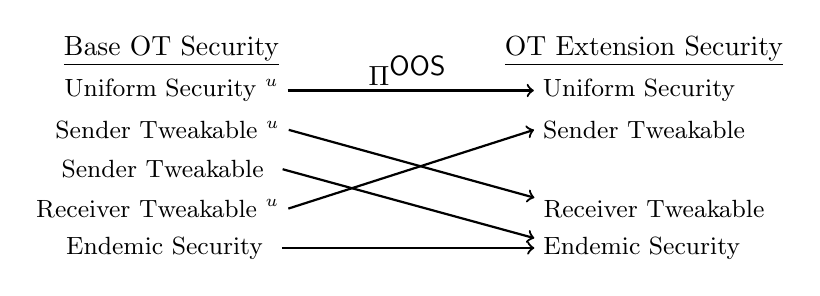
\begin{tikzpicture}[scale=0.5]\small
	\node (pi) at (6,4.5) {\normalsize $\Pi^\textsf{OOS}$};
	\node (Base) at (0,5) {\underline{\normalsize Base OT Security}};
	\node (U) at (0,4) {Uniform Security $\OOT^{\U u}$};
	\node (SCu) at (-0.1,3) {Sender Tweakable $\OOT^{\send u}$};
	\node (SC) at (-0.1,2) {Sender Tweakable $\OOT^{\send}$};
	\node (RC) at (-0.35,1) {Receiver Tweakable  $\OOT^{\rec u}$};
	\node (E) at (-0.05,0) {Endemic Security  $\OOT^{\E}$};
	
	
	\node (Ext) at (12,5) {\underline{\normalsize OT Extension Security}};
	\node (EU) at (12,4) {Uniform Security $\OOT^{\U}$};
	\node (ESC) at (12.13,3) {Sender Tweakable $\OOT^{\send}$};
	\node (ERC) at (12.38,1) {Receiver Tweakable  $\OOT^{\rec}$};
	\node (EE) at (12.07,0) {Endemic Security  $\OOT^{\E}$};
%	\draw [-implies,double equal sign distance] (U) -- (SC);
%	\draw [-implies,double equal sign distance] (U) -- (RC);
%	\draw [-implies,double equal sign distance] (SC) -- (E);
%	\draw [-implies,double equal sign distance] (RC) -- (E);
	\draw [->, thick] (U) -- (EU);
	\draw [->, thick] (E) -- (EE);
	\draw [->, thick] (SCu.east) -- (ERC.175);
	\draw [->, thick] (RC.east) -- (ESC.west);
	\draw [->, thick] (SC.east) -- (EE.175);
	
%	\draw [-, thick] (5,2.5)-- (TC);
%	\draw [->, thick] (E) .. controls (1,0.75) .. (SC);
%	\draw [->, thick] (E) .. controls (7,0.75) .. (RC);
	\end{tikzpicture}
	\label{fig:OTExtrelations}
	\caption{
		The figure depicts the implication different Base OT security notions have on the result OT extension protocol.  $A\rightarrow B$ denotes that any OT realizing security $A$ can be efficiently transformed by $\Pi^\textsf{OOS}$ (\definitionref{def:OOS}) into an OT realizing security $B$.
	}
\end{figure}


The functionality of 1-out-of-$N$ OT extension ...

We begin by reviewing the protocol of Orr\'u, Orsini and Scholl\cite{OOS16} with some cosmetic differences to aid presentation. \definitionref{def:OOS} in conjunction with \figureref{fig:otExt}, \ref{fig:OChallenge} defines the \cite{OOS16} protocol. 

...

\begin{definition}\label{def:OOS}
	Let $\Pi^{\textsf{OOS}}$ be the protocol of \figureref{fig:otExt} where $\O^{\textsf{chllng}}:=\Pi^{\textsf{chllng}}$ (\figureref{fig:OChallenge}) and $\OOT:=\OOT^\send$ (\definitionref{def:ot}), i.e.  \cite[Protocol 2]{OOS16}.
\end{definition}



\subsection{OT Extension Attacks}


\begin{lemma} 
	There exists a ppt adversary $\Adv$ and distinguisher $D$ such that for any $\Adv'$ 
	$$
		|\Pr[D((\Adv, \rec)_{\langle\Adv,\rec\rangle})=1]-\Pr[D((\Adv', \O^{\E}_{\textsf{OT,\rec}})_{\langle\Adv',\O^{\E}_{\textsf{OT}}\rangle})=1]|=1-\negl
	$$
	where $\langle\Adv,\rec\rangle$ is the $\Pi^{\textsf{OOS}}$ protocol (\definitionref{def:OOS}), $\O^{\E}_{\textsf{OT,\send}}$ is the \send's side output within the view of $\OOT^{\E}$ and all algorithms additionally receive input $1^\kappa$. 
\end{lemma}
\begin{proof} 
	For simplicity let $N=2$ and $m=\kappa$. We define $\Adv$ as follows. $\Adv$ plays the role of \send and replaces the input to $\OOT^\send$, the receiver input, with the string $b:=\{0\}^\nc$. \Adv outputs the matrix $Q$.
	
	We define $D$ as follows. $D$ samples the selection bits $x_1,...,x_m\gets\{0,1\}$ and sends them to \rec. $D$ executes $\Adv$ who outputs $Q$ and \rec outputs $\vv_{x_1,1},...,\vv_{x_m,m}$. If $\vv_{x_i,i}=\H(i,\qq_i)$ for $i\in[m]$, output 1, otherwise 0. In the real interaction it clearly holds that $\Pr[D((\Adv, \rec)_{\langle\Adv,\rec\rangle})=1]=1$ since $\qq_i=\tt_i$.
	
	By definition the input of $\Adv'$ is independent of $x_i$ and receives no output from $\OOT^\E$ (apart from their input $(\vv_{0,i},\vv_{1,i})_{i\in [m]}$). Therefore, it must hold that $\Pr[D((\Adv', \rec)_{\langle\Adv',\O^{\E}_{\textsf{OT,\send}}\rangle})=1]=2^{\kappa}$.
\end{proof}


\begin{lemma} 
	There exists a ppt adversary $\Adv$ and distinguisher $D$ such that for any $\Adv'$ 
	$$
	|\Pr[D((\send, \Adv)_{\langle\send, \Adv\rangle})=1]-\Pr[D((\O^{\U}_{\textsf{OT,\send}}, \Adv')_{\langle\OOT^\U, \Adv'\rangle})=1]|=1-2^{-\kappa}
	$$
	where $\langle\send, \Adv\rangle$ is the $\Pi^{\textsf{OOS}}$ protocol (\definitionref{def:OOS}), $\O^{\U}_{\textsf{OT,\send}}$ is the \rec's side output within the view of $\OOT^{\U}$ and all algorithms additionally receive input $1^\kappa$. 
\end{lemma}
\begin{proof}
	For simplicity let $N=2$ and $m=1$. We define $\Adv$ as follows. $\Adv$ plays the role of \rec and replaces the input to $\OOT^\send$, the sender input, with strings $\tt_0^j,\tt_1^j\in \{0\}^{m'}$ and then completes the protocol as normal.
	
	We define $D$ as follows. $D$ executes \send and \Adv with input $x_1=0$. \send outputs $(\vv_{0,1},\vv_{1,1})$ and $D$ outputs 1 if $\vv_{0,1}=\H(1, \{0\}^\nc)$ and 0 otherwise. In the real interaction it clearly holds that $\Pr[D((\send, \Adv)_{\langle\send, \Adv\rangle})=1]=1$. In the ideal interaction the honest \send will output a uniformly distributed $\vv_{0,1}\in\{0,1\}^\kappa$ which was sampled by $\OOT^{\U}$ and therefore $\Pr[D((\send, \Adv')_{\langle\O^{\U}_{\textsf{OT,\rec}}, \Adv'\rangle})=1]=2^{-\kappa}$.
\end{proof}



\begin{figure}[t]
	\framebox{\begin{minipage}{0.95\linewidth}\small
			\textsc{Parameters:} $\kappa$ is the computational security parameter. $m$ denotes the number of OTs. $N$ denotes the number of messages each OT has. $\mathcal{C}$ is an $[\nc,\kc,\dc]$ binary linear code such that $\kc=\log_2 N$ and $\dc\geq \kappa$.\\
			\textsc{Requirements:} $\H : [m] \times \mathbb{F}_2^\nc \rightarrow \mathbb{F}_2^\kappa$ 
			%and $\H' : \mathbb{F}^{(m+\kappa)\times \nc}_2 \rightarrow \mathbb{F}^{m\times \kappa}_2$ are 
			is a random oracle. % and $\PRG : \{0,1\}^{\kappa} \rightarrow \{0,1\}^{m+\kappa}$ is a pseudorandom generator. 
		
			$\O^{\textsf{chllng}} : \mathbb{F}^{(m+s)\times \nc}_2 \rightarrow \mathbb{F}^{m\times s}_2$ is an oracle that returns a challenge string to both parties. Let $m'=m+s$. 	$\OOT$ is an 1-out-of-2 OT oracle with output messages in $\mathbb{F}_2^{m'}$.
			\\
			
			\begin{enumerate}
				\item Both parties invoke $\nc$  instances of $\OOT$  where \send takes the role of the receiver. If $\OOT$ has inputs, the corresponding party  locally samples them uniformly from the input domains. \send receives $(\bb\in\{0,1\}^\nc, \{\tt^j_{b_j}\}_{j\in [\nc]})$. \rec receives $\{(\tt^j_0,\tt^j_1)\}_{j\in [\nc]}$. Let $T_0\in \mathbb{F}^{m'\times \nc}_2$ denote the matrix formed by concatenating the column vectors $\tt^0_0||...||\tt^\nc_0$. \\
			
%				\item \rec constructs matrices $T_0,T_1\in \mathbb{F}^{m'\times \nc}_2$ from the seeds $\{(\rr^j_0,\rr^j_1)\}_{j\in [\nc]}$ so that the respective columns are:
%				$$
%					\tt^j_0 := \PRG(\rr^j_0)\in \mathbb{F}^{m'}_2,\qquad \tt^j_1 := \PRG(\rr^j_1)\in \mathbb{F}^{m'}_2,\qquad \forall j\in[\nc]
%				$$
%				In the same way \send produces $\tt^j_{b_j}$, for each $j\in[\nc]$. Summarizing, \rec holds $\{(\tt^j_0,\tt^j_1)\}_{j\in[\nc]}$ and \send holds $\{\tt^j_{b_j}\}_{j\in[\nc]}$.
%				
				\item \rec samples random $\ww_{m+\ell}\gets \mathbb{F}^\kc_2$, for $\ell\in[s]$, and then constructs a matrix $C\in\mathbb{F}^{m'\times \nc}_2$ such that each row $\cc_i$ is the codeword $\mathcal{C}(\ww_i)$. Then, \rec sends to \send the values
				$$
					\uu^j :=\tt^j_0 +\tt^j_1+\cc^j, \qquad \forall j\in[\nc],
				$$
				where $\cc^j$ is the $j$-th column of $C$.
				
				\item \send receives $\uu^j\in\mathbb{F}^{m'}_2$ and computes
				$$
					\qq^j := b_j \cdot \uu^j +\tt^j_{b_j} = b_j\cdot \cc^j+\tt^j_0,\qquad \forall j\in[\nc]
				$$
				that form the columns of an $(m'\times \nc)$ matrix $Q$. Denoting the rows of $T_0, Q$ by $\tt_i,\qq_i$, \rec now holds $\cc_i,\tt_i$ and \send holds $\bb, \qq_i$ so that 
				$$
					\qq_i = \cc_i\odot \bb+\tt_i,\qquad \forall i\in[m'].
				$$
				
				\item \emph{Consistency check:}
				\begin{itemize}
					\item Both parties query the challenge oracle $\O^{\textsf{chllng}}$ on input $u^j$ for $j\in[\nc]$  which samples and returns $X=\{(x_1^{\ell}, ...,x_m^{\ell} )\in \mathbb{F}^m_2\}_{\ell\in[s]}$ % := H'(\uu^1|| ... || \uu^\nc).
					to both parties.
					
					\item \rec computes and sends, for $\ell \in[s]$:
					$$
						\widehat \tt^{\ell} := \sum_{i\in[m]} \tt_i \cdot x_i^\ell + \tt_{m+\ell}, \qquad \widehat \ww^\ell := \sum_{i\in[m]} \ww_i \cdot x_i^\ell + \ww_{m+\ell}
					$$
					
					\item \send computes $\widehat \qq^\ell := \sum_{i\in[m]} \qq_i \cdot x^\ell_i + \qq_{m+\ell}$, and checks that:
					$$
						\widehat\tt^\ell + \widehat\qq^\ell = \mathcal{C}(\widehat\ww^\ell) \odot \bb, \qquad \forall\ell\in[s].
					$$
					If the check fails, \send sends $\textsf{Abort}$, and otherwise continues.
				\end{itemize}
			\end{enumerate}
		
		\textbf{Output:} \send outputs $\vv_{\ww,i}:=\H(i,\qq_i+\mathcal{C}(\ww)\odot \bb), \forall i\in[m]$ and $\ww\in S_i$. \rec outputs $\vv_{\ww,i}:= \H(i,\tt_i), \forall i\in[m]$.
	\end{minipage}}
	\caption{ 1-out-of-$N$ OT Extension.}
	\label{fig:otExt}
\end{figure}


\begin{figure}[t]
	\framebox{\begin{minipage}{0.95\linewidth}\small
			\textsc{Parameters:} $\lambda$ is the statistical security parameter.
			
			\textbf{Inputs:} \send inputs $U\in\mathbb{F}^{(m+\lambda)\times n}_2$ and \rec inputs $U'$.
			\begin{enumerate}
				\item \send uniformly samples $X\gets \mathbb{F}^{m\times n}_2$ and sends it to \rec.
				\item Both parties output $X$.
			\end{enumerate}
	\end{minipage}}
	\caption{ Challenge Protocol $\Pi^\textsf{chllng}$ implementing $\O^\textsf{chllng}$.}
	\label{fig:OChallenge}
\end{figure}


